\documentclass[a4paper, 12pt]{article}
\usepackage[top=2cm, bottom=2cm, left=1.5cm, right=1.5cm]{geometry}
\usepackage[utf8]{inputenc}
\usepackage{amsmath, amsfonts, amssymb}
\usepackage{graphicx}
\usepackage[brazil]{babel}
\usepackage{indentfirst}
\usepackage[small,bf]{caption}



\begin{document}
%%%%%%%%%%%%%%%%%%%%%%%%%%%%%%%%Começo do documento%%%%%%%%%%%%%%%%%%%%%%%%

\thispagestyle{empty}
\begin{titlepage}
 \vfill
  \begin{center}
   {\large \textbf{UNIVERSIDADE ESTADUAL DE CAMPINAS}} \\[3cm] %Não precisa mudar o nome da Universidade

   {\large Lucas Jacinto Gonçalves RA: 240013 }\\[0.25cm] %Não precisa mudar nossos nomes
   {\large Leonardo Novaes do Nascimento RA: 220142 }\\[0.25cm]
   {\large Jorge Henrique de Andrade Pacheco Reis RA: 237966 }\\[5.5cm]


   {\Large Relatório do experimento 5: Calorimetria}\\[6cm] %Mudar o título do trabalho, conforme necessário

   \hspace{.45\textwidth} %posiciona a minipage
   \begin{minipage}{.5\textwidth}
   \large Relatório do experimento 5, da disciplina de Física Experimental 2, F 229.\\[1cm]
Professor Dr. Ricardo Urbano.		%Se quisermos colocar o nome do professor...
  \end{minipage}
  \vfill

\vspace{2cm}

\large Campinas, novembro de 2019. 	%Mudar data, conforme necessário.


\end{center}

\end{titlepage}



\pagebreak




\textbf{Resumo}
\\

Ao estudar processos termodinâmicos, muitas vezes é necessário a quantização das troca de energia, na forma de calor, de um dado processo físico ou químico. Por isso é fundamental que um dado processo quando for analisado as trocas de energia seja feito em um espaço termodinamicamente isolado para que não ocorra troca de energia com o ambiente externo (ao redor).

Na quantização da energia trocada na forma de calor, quando corpos a diferentes temperaturas são colocados em contato e entram em equilíbrio térmico, queremos analisar Q que é a energia transferida na forma de calor para ou de um corpo de massa m, por meio de seu resfriamento ou aquecimento, estando relacionada com a variação de sua temperatura através da equação: 
\\
\\
$$Q = C \Delta T = mc \Delta T, $$
\\
onde $C$ é a \textit{capacidade térmica} de um objeto e $c$ é o \textit{calor específico} de um objeto.

		\begin{figure}[!h]
		\centering
		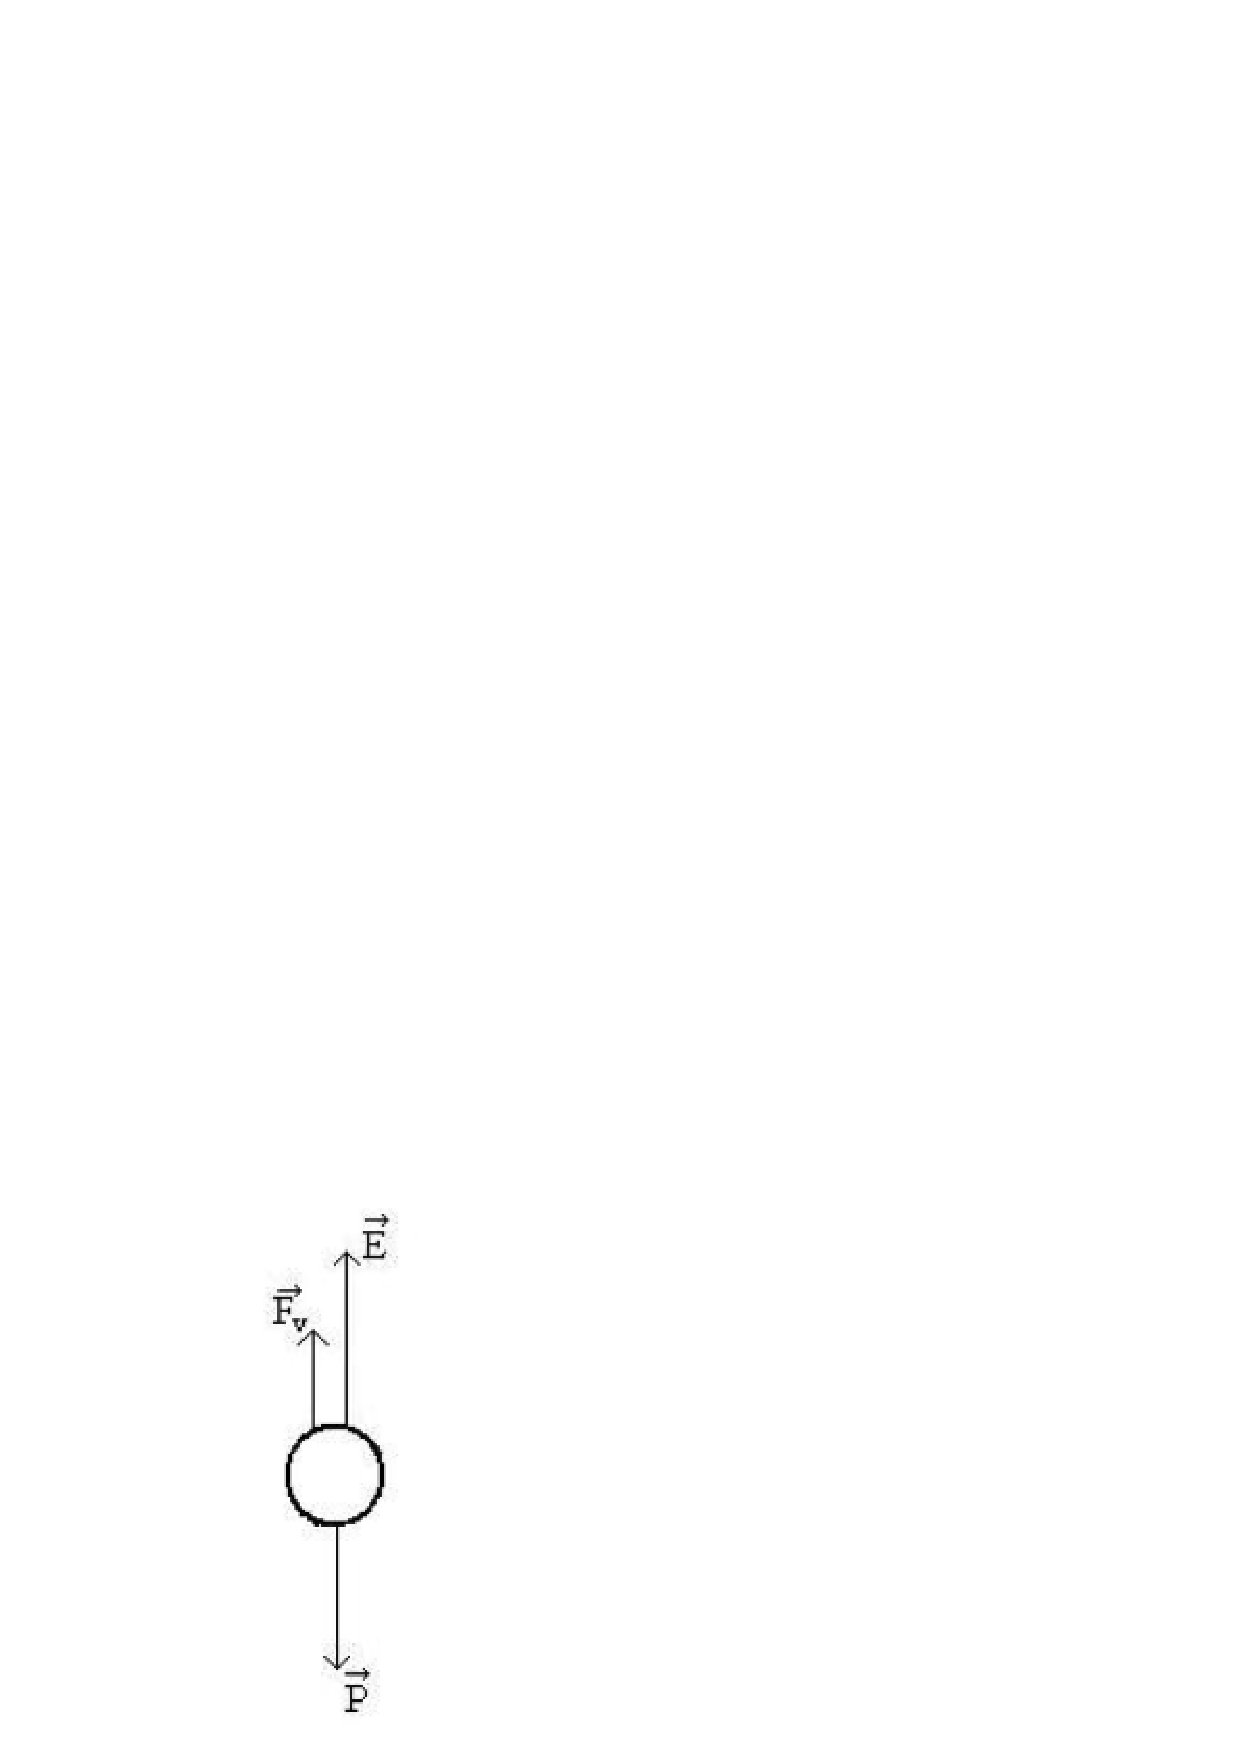
\includegraphics[scale = 0.45]{fig1.png}
		%\caption{}
		\end{figure}

\pagebreak



\textbf{Procedimentos e incertezas}
\\

Para esse procedimento utilizamos os seguintes aparatos: chaleira elétrica, calorímetro, água, termômetro de álcool, termopar, milivoltímetro, blocos de cobre, chumbo e alumínio, garrafa térmica com gelo, cronômetro e balança de precisão.

\begin{figure}[!h]
		\centering
		\includegraphics[scale = 0.50]{tabela1.png}
		%\caption{}
		\end{figure}

\begin{figure}[!h]
		\centering
		\includegraphics[scale = 0.50]{tabela2.png}
		%\caption{}
		\end{figure}

Para esse experimento dividimos o procedimento em três partes: Na primeira parte fizemos medições da tensão gerada por um termopar sendo que um lado estava  a 0ºC e o outro lado a temperatura foi variada (ambos estavam em porções de água). 

Na segunda parte do experimento foi calculado a capacidade térmica do calorímetro utilizando para isso a lei de conservação de energia, para o cálculo da capacidade térmica do calorímetro foi necessário misturar duas porções de água a diferentes temperaturas no calorímetro afim de que atingissem o equilíbrio térmico.

A terceira e última parte do experimento foi calculada o calor específico de três metais diferentes: cobre, chumbo e aço. Para esse procedimento, cada metal foi colocado por um intervalo de tempo em água com temperatura elevada e logo em seguida, foi colocado no calorímetro juntamente com água a temperatura ambiente para que fosse atingido o equilíbrio térmico para obtenção da temperatura final. Com esses dados, e utilizando a lei de conservação de energia, obtivemos ferramental para cálculo do calor específico  de cada metal.


\pagebreak


\textbf{Resultados}
\\

\underline{Na primeira parte do experimento}, foram feitas 4 medidas a fim de montar um gráfico da Tensão do voltímetro em função da diferença de temperatura no termopar (V(t)):
Os resultados obtidos experimentalmente estão na tabela a seguir:

\begin{figure}[!h]
		\centering
		\includegraphics[scale = 0.50]{tabela3.png}
		%\caption{}
		\end{figure}

Com isso, pode-se obter um gráfico de (V(t)):
\\

\begin{figure}[!h]
		\centering
		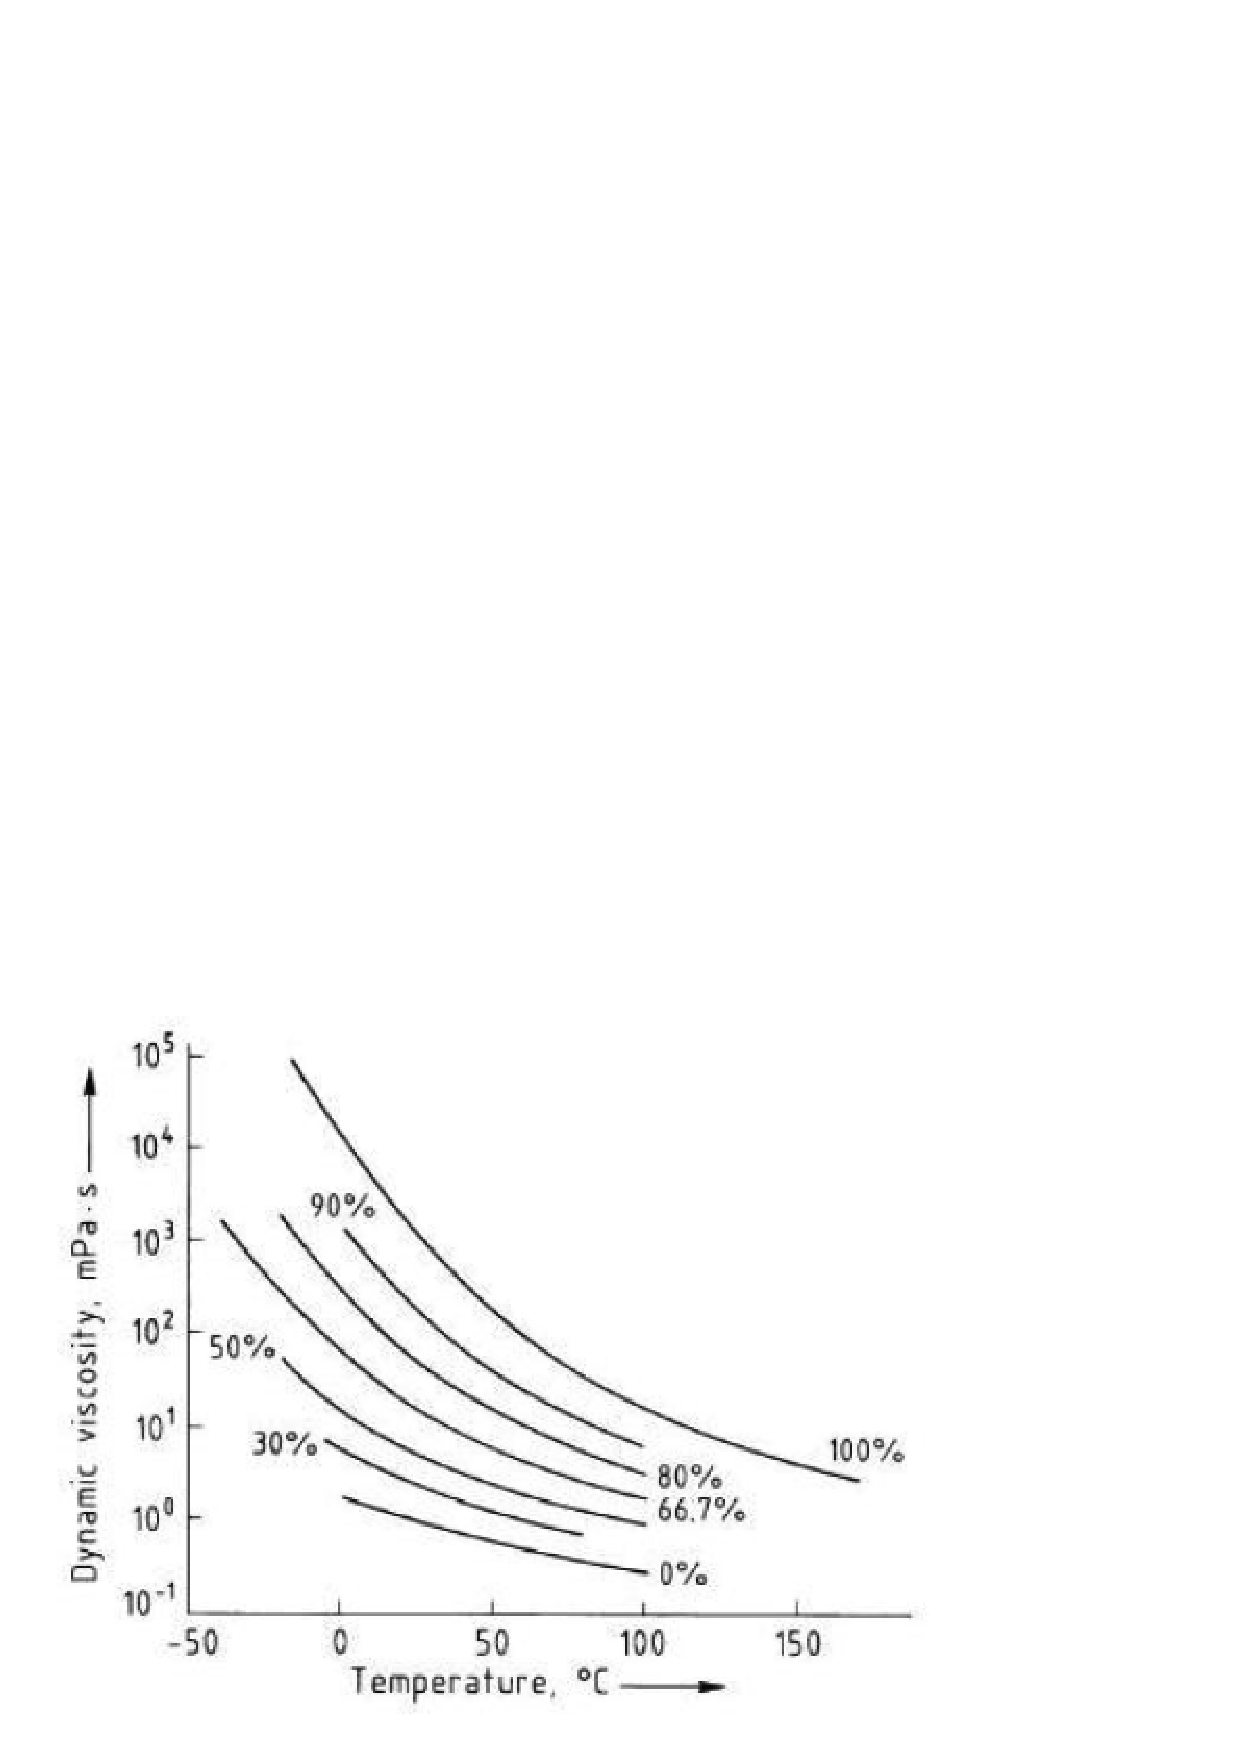
\includegraphics[scale = 0.50]{fig2.png}
		%\caption{Gráfico 1}
		\end{figure}

Com isso obtemos um coeficiente angular $a = 0,0575 \, \pm \, 0,0005 \, \,  mVºC^{-1}$ e um coeficiente linear $b = -0,34 \, \pm \, 0,03 \, \, ºC$. A partir de agora o coeficiente angular e o linear serão usados como os fatores de conversão entre a leitura do voltímetro e a diferença de temperatura.
\\

\underline{Na segunda parte do experimento}, a equipe calculou o valor da capacidade térmica do calorímetro. Foi usada uma porção de água a $T_1 = 29 \,  \pm  \, 0,2 \, \, ºC$  de $m_1 = 194,7 \,  \pm  \, 0,04 \, \, g$ e outra a $T_2 = 80 \pm 0,2 \, \, ºC$ de $m_2 = 46,4 \pm 0,04 \, \, g$. A temperatura inicial do calorímetro foi considerada como a temperatura ambiente, igual a temperatura de uma das porções de água $29 \pm 0,2 \, \, ºC$. Após a mistura e o equilíbrio térmico do conjunto o voltímetro mostra $2,34 \pm 0,01 \, \, mV$ que, segundo o fator de conversão encontrado pela equipe, é $T = 46,6 \pm 0,7 \, \, ºC$. Por fim, com a \textit{Lei Zero da Termodinâmica}, e com o calor específico da água $c = 1 \, \, cal \, g^{-1} \, ºC^{-1}$ pode-se montar uma expressão para calcular a capacidade térmica do calorímetro, encontrada abaixo:

$$ C = \dfrac{- c m_1 (T - T_1)  - c m_2 (T - T_2)}{T - T_1}$$

O valor encontrado experimentalmente para a capacidade térmica é $C = -107 \pm 5 \, \, cal \, g^{-1} \, ºC^{-1}$.

\pagebreak

\underline{Na terceira parte do experimento}, usamos a mesma lógica da segunda parte do experimento, a equipe usou a lei da conservação de energia e o calor específico da água $c = 1 \, \, cal \, g^{-1} \, ºC^{-1}$ para montar uma expressão para calcular o calor específico do metal, encontrada abaixo:

$$ c_m = \dfrac{- C (T - T_1)  - c m_a (T - T_1)}{m_m (T - T_q)} $$

Sendo $c_m$ o calor específico do metal, $T$ a temperatura final do conjunto, $T_1$ a temperatura inicial do calorímetro e da água, $m_a$ massa de água, $T_q$ a temperatura inicial do metal e $m_m$ a massa do metal.
Colocando os valores encontrados experimentalmente na tabela a seguir:

\begin{figure}[!h]
		\centering
		\includegraphics[scale = 0.55]{tabela4.png}
		%\caption{}
		\end{figure}
Colocando esses valores na expressão obtemos que o seguinte:

\begin{figure}[!h]
		\centering
		\includegraphics[scale = 0.55]{tabela5.png}
		%\caption{}
		\end{figure}

\pagebreak


\textbf{Discussão}

Na primeira parte do experimento foi encontrado o fator de conversão da leitura do voltímetro para a diferença de temperatura entre os fios do termopar. Pode-se comparar esse fator com a tabela de calibração dada pelo Moodle.

\begin{figure}[!h]
		\centering
		\includegraphics[scale = 0.55]{tabela6.png}
		%\caption{}
		\end{figure}


Logo, vemos que o valor encontrado experimentalmente não bate com o previsto, porém com uma maior incerteza poderíamos englobar o valor modelo.

Por fim, na terceira parte do experimento, obtivemos os valores dos calores específicos de cada metal e procurando na internet obtemos os valores de referência: 
\\

Cobre $= 0,094 \, \, cal \, g^{-1} \, ºC^{-1}$.

(https://www.materiais.gelsonluz.com/2018/09/calor-especifico-do-cobre.html)
\\


Chumbo $= 0,031 \, \, cal \, g^{-1} \, ºC^{-1}$.

(https://www.materiais.gelsonluz.com/2018/09/calor-especifico-do-chumbo.html) 
\\

Aço $= 0,12 \, \, cal \, g^{-1} \, ºC^{-1}$.

(https://www.materiais.gelsonluz.com/2018/09/calor-especifico-do-aco.html)
\\
\\

No caso do cobre e do aço, os valores de referência estão de acordo com os obtidos no experimento, no caso do chumbo um pequeno aumento da incerteza poderia colocar os valores em acordo.
\\

Nota: Obtivemos um valor negativo para a capacidade térmica do calorímetro e  mediante algumas discussões com os membros da equipe pudemos supor que alguns fatores influenciaram esse resultado: em primeiro lugar tivemos um problema sério com relação ao tempo, já que nosso milivoltímetro com o termopar não estava calibrando corretamente, onde perdemos muito tempo; 
em segundo lugar, a questão do equilíbrio térmico do sistema, que não tínhamos como saber com exatidão se havia ocorrido, o que comprometia a qualidade do experimento e, semelhante, imperfeições/ineficiências de construção no calorímetro; 
em terceiro lugar, os resultados dos calores específicos do aço e do chumbo aparentemente "trocados" \, indica que, embora o intervalo de incerteza "cubra", pode ser que tenhamos nos equivocado com relação a \textit{qual peça correspondia a qual material} e;
em quarto lugar, o fato de que a mistura de gelo e água na referência a 0 ºC não estarem exatamente nessa temperatura $-$ tendo em vista que o gelo acabou muito rápido no dia do experimento $-$ e o "transporte" dos metais do recipiente de água quente para o calorímetro, que deu certa resfriada nele, mudando a temperatura. 


\pagebreak


\textbf{Anexos}



%%%%%%%%%%%%%%%%%%%%%%%%%%FIM%%%%%%%%%%%%%%%%%%%%%%%%%%%5
\end{document}